\documentclass{beamer}
\usepackage{multimedia}


%===Pick Theme===
\usetheme{Warsaw}
\usecolortheme{beaver}
\useoutertheme{infolines}
\useinnertheme{circles}

%===Customize Theme=== %
\setbeamercolor{item}{fg=darkred}
\setbeamertemplate{itemize subitem}{$\circ$}
\setbeamercolor*{block title}{fg=white, bg=darkred}
\setbeamercolor*{block body}{bg=lightgray}

%===Set the covered style=== %
\setbeamercovered{transparent}
%===Set the bib reference key style=== %
\setbeamertemplate{bibliography item}[text]
%===Disable navigation bar=== %
\setbeamertemplate{navigation symbols}{}%remove navigation symbols

\usepackage{minted}
\setminted[python]{bgcolor=bg,fontsize=\scriptsize,linenos}
\setmintedinline[python]{bgcolor=bg,fontsize=\scriptsize}
\setmintedinline[bash]{bgcolor=bg,fontsize=\scriptsize}
\setminted[xml]{bgcolor=bg,fontsize=\scriptsize,linenos}
\setmintedinline[xml]{bgcolor=bg,fontsize=\scriptsize}
\newcommand{\pyinline}[1]{\mintinline{python}{#1}}
\newcommand{\bashinline}[1]{\mintinline{bash}{#1}}
%===Logos=== %

%\usepackage{pgf}
%\logo{\pgfputat{\pgfxy(-1,7)}{\pgfbox[center,base]{
\includegraphics[height=0.5in]{fig/duckietown_logo}}}}

\logo{
\includegraphics[height=0.5in]{fig/duckietown_logo}}
\titlegraphic{ %
\centering

\includegraphics[height=1.5in]{fig/duckietown_logo}%\hspace{2ex}
%\raisebox{-0.75in}{
\includegraphics[height=1.5in]{fig/indigoigloo_600.png}}
} %


\author[Shih-Yuan Liu]{Shih-Yuan Liu}
\title[ROS in Duckietown]{Robot Operating System (ROS) in Duckietown}
\institute[Duckietown MIT]{Duckietown, MIT}
\date[Feb. 16th, 2016]{February 16th 2016}

\begin{document}
\definecolor{bg}{rgb}{0.95,0.95,0.95}

\begin{frame}[plain,label=titlepage,noframenumbering] %[plain,noframenumbering] will not show the header and footer
	\titlepage
\end{frame}

\begin{frame}[label=overview]{Overview}
	\tableofcontents
	%\tableofcontents[sectionstyle=show/shaded,subsectionstyle=show/shaded/shaded]
\end{frame}


\section{Introduction}

\begin{frame}{What is ROS?}
\begin{columns}
	\begin{column}{0.55\textwidth}
		Robotics Operating System (ROS) is an \alert{open-source}, \alert{meta-operating system} for your \alert{robot}:
		\begin{itemize}
			\item Hardware abstraction and low-level device control
			\item Message-passing between processes
			\item Package and build management system
			\item Data visualization, logging, and analysis
		\end{itemize}
	\end{column}
	\begin{column}{0.45\textwidth}
		\centering
		
\includegraphics[width=\textwidth]{fig/indigoigloo_600.png}
	\end{column}
\end{columns}
\end{frame}

\begin{frame}{Why ROS?}
\begin{columns}
	\begin{column}{0.55\textwidth}
		\begin{itemize}
			\item Open-source
			\item Well documented
			\item \alert{\texttt{python}} for accessibility and \alert{\texttt{C++}} for performance 
			\item Native to \alert{Ubuntu}
			\item Active community with \alert{3000+} packages
		\end{itemize}
	\end{column}
	\begin{column}{0.45\textwidth}
		\centering
		
\includegraphics[width=\textwidth]{fig/indigoigloo_600.png}
	\end{column}
\end{columns}
\onslide<2>{
\begin{block}{Is there a ROS package for $x$? Can ROS do $y$?}
	Most likely YES!
\end{block}}

\end{frame}

\section{Concept Overview}

% \subsection{Packages}
\begin{frame}{Packages}
\begin{columns}
	\begin{column}{0.6\textwidth}
		\begin{itemize}
			\item Packages are used to organize:
			\begin{itemize}
				\item Modules
				\item Build and runtime dependencies
				\item Namespaces
			\end{itemize}
			\item Key Files
				\begin{itemize}
					\item CMakeLists.txt
					\item package.xml
					\item setup.py
				\end{itemize}
			\item Tools
				\begin{itemize}
					\item \mintinline{bash}{roscd}
					\item \mintinline{bash}{rospack profile}
					\item \mintinline{bash}{rospack depends}
				\end{itemize}
		\end{itemize}
	\end{column}
	\begin{column}{0.4\textwidth}
		\centering
		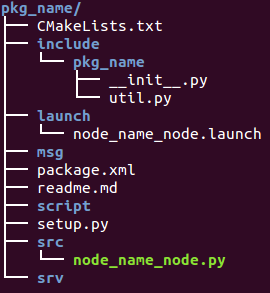
\includegraphics[width=\textwidth]{fig/pkg_tree.png}
	\end{column}
\end{columns}
\end{frame}

% \subsection{Nodes and Topics}
\begin{frame}{Nodes and Topics}
	\begin{columns}
		\begin{column}{0.6\textwidth}
			\begin{itemize}
				\item Nodes are:
					\begin{itemize}
					\item Exectuables
					\item Each its own process
					\item Publishes/Subscribes to Topics
					\end{itemize}
				\item Topics:
					\begin{itemize}
					\item Passes information between nodes
					\item Topic type defined by messages
					\item One-to-many/Many-to-one
					\end{itemize}
				\item Tools:
					\begin{itemize}
					\item \mintinline{bash}{rqt_graph}
					\item \mintinline{bash}{rosnode list}
					\item \mintinline{bash}{rosnode info}
					\item \mintinline{bash}{rostopic info}
					\item \mintinline{bash}{rostopic list}
					\end{itemize}
			\end{itemize}
		\end{column}
		\begin{column}{0.4\textwidth}
			\centering
			TODO: Node -> Topic -> Node figure
			TODO: Demo with Duckiebot joystick.launch.
		\end{column}
	\end{columns}
\end{frame}

\begin{frame}{ROS Master}
	\begin{columns}
		\begin{column}{0.6\textwidth}
			\begin{itemize}
			\item Handles communication between nodes
			\item Connects publisher and subscriber
			\item Traffic does \alert{not} go through the master once connected
			\item TCP/IP connection (UDP option available)
			\end{itemize}
		\end{column}
		\begin{column}{0.4\textwidth}
			\centering
			TODO: operator picture\\
			TODO: Connection graph
		\end{column}
	\end{columns}
\end{frame}

\begin{frame}{Messages}
	\begin{columns}
		\begin{column}{0.6\textwidth}
			\begin{itemize}
				\item Define types of Topic
				\item Basics types: \bashinline{bool}, \bashinline{string}, \bashinline{float}, etc
				\item \bashinline{Header} contains \bashinline{stamp} and \bashinline{frame_id} and is recommended for every message
				\item Use composition of existing messages when possible
					\begin{itemize}
						\item \bashinline{std_msgs}, \bashinline{geometry_msgs}, \bashinline{sensor_msgs}, \bashinline{nav_msgs}, \bashinline{visualization_msgs}
					\end{itemize}
				\item \bashinline{duckietown_msgs} contains all customized messages for Duckietown.
				\item Tool: \mintinline{bash}{rosmsg show}
			\end{itemize}
		\end{column}
	\begin{column}{0.4\textwidth}
		\centering
		TODO: couple of example messages definition (WheelsCmdStamped)

		DEMO: use rosmsg show to show the definition of a couple of msgs
		\end{column}
	\end{columns}
\end{frame}

\begin{frame}{Parameters}
	\begin{columns}
		\begin{column}{0.6\textwidth}
			\begin{itemize}
				\item Nodes can set/get parameters to/from the parameter server
				\item Parameters can be changed during run time
				\item Parameters can be load/dump to yaml files 
				\item Provides simple parameterization of nodes
				\item Tools:
					\begin{itemize}
						\item \bashinline{rosparam list}
						\item \bashinline{rosparam get/set}
						\item \bashinline{rosparam load/dump}
					\end{itemize}
			\end{itemize}
		\end{column}
	\begin{column}{0.4\textwidth}
		\centering
		TODO: Parameter example of camera.launch and joystick.launch
		%\includegraphics[width=\textwidth]{}
		\end{column}
	\end{columns}
\end{frame}

\begin{frame}{Launch Files}
	\begin{columns}
		\begin{column}{0.6\textwidth}
			\begin{itemize}
				\item ROS specific scripts as XML
				\item Capabilities:
					\begin{itemize}
						\item Launch nodes
						\item Set node names
						\item Set/Load parameters
						\item Remap topics
						\item Specify machines
						\item Configuration at launch time through \bashinline{<arg>}
					\end{itemize}
				\item Tools:
					\begin{itemize}
						\item \bashinline{roslaunch --args}
						\item \bashinline{roslaunch --find}
						\item \bashinline{roslaunch --ros-args}
					\end{itemize}
				\item In Duckietown:
					\begin{itemize}
						\item Each node has one elemental launch file
						\item Documents the I/O of a node
						\item Standard interfaces through \bashinline{<arg>}
					\end{itemize}
			\end{itemize}
		\end{column}
	\begin{column}{0.4\textwidth}
		\centering
		TODO: example using camera.launch and joystick.launch
		DEMO: command line argument --args --ros-arg --find etc
		%\includegraphics[width=\textwidth]{}
		\end{column}
	\end{columns}
\end{frame}

\begin{frame}{Services}
	TODO
\end{frame}

\section{Duckietown ROS Diagram}

\begin{frame}{Duckietown ROS Architecture}
\begin{itemize}
	\item TODO:Control
	\item TODO:Perception
	\item TODO:Localization
	\item TODO:Planning and coordination
\end{itemize}
\end{frame}

% \begin{frame}{Duckietown ROS guidelines}
% \end{frame}

\begin{frame}{Resources}
  \begin{columns}
    \begin{column}{0.6\textwidth}
      \begin{itemize}
        \item TODO: links to ROS tutorial and wiki
      \end{itemize}
    \end{column}
  \begin{column}{0.4\textwidth}
    \centering
    %\includegraphics[width=\textwidth]{}
    \end{column}
  \end{columns}
\end{frame}

%\begin{frame}{Snippet}
%	\begin{itemize}[<+->]
%		\item Hey
%		\inputminted{python}{snippet/test.py}
%		\item Ho \mintinline{python}{import numpy as np}
%	\end{itemize}
%\end{frame}

\end{document}